\documentclass[crop,convert={outext=.svg,command=\unexpanded{pdf2svg \infile\space\outfile}},multi=false]{standalone}[2012/04/13]
%\usetikzlibrary{...}% tikz package already loaded by 'tikz' option

\usepackage[dvipsnames]{xcolor}
\usepackage{tikz}
\usetikzlibrary{arrows.meta,graphs,decorations.pathmorphing,backgrounds,positioning,fit,
  petri,shapes,calc,matrix,trees,shadows,shapes.symbols}
\tikzset{
  pre/.style={<-,shorten <=1pt,>={Stealth[round]},semithick},
  post/.style={->,shorten >=1pt,>={Stealth[round]},semithick},
  bidir/.style={<->,shorten <=1pt,>={Stealth[round]},semithick},
}
\usepackage{ebgaramond}



\makeatletter
\begin{document}
   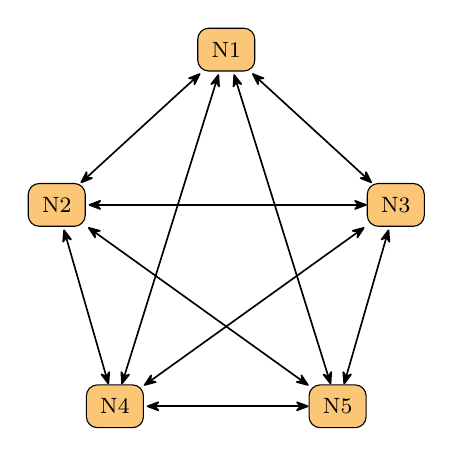
\begin{tikzpicture}[
        replica/.style={rectangle,rounded corners, draw=black, inner sep=5pt,
        minimum height=10, minimum width=12, align=center,fill=YellowOrange!50,
        font={\footnotesize} },
        client/.style={rectangle,rounded corners,inner sep=5pt, minimum size=15, align=center,
        draw=black,fill=ProcessBlue!50},
        node distance=2cm
        ]
    
        \node[replica] (n1) {N1};
        \node[replica, below left=of n1] (n2) {N2};
        \node[replica, below right=of n1]  (n3) {N3};
        \node[replica, below right=2cm and 0cm of n2]  (n4) {N4};
        \node[replica, below left=2cm and 0cm of n3]  (n5) {N5};
    
        \path[bidir] (n1) edge (n2);
        \path[bidir] (n1) edge (n3);
        \path[bidir] (n1) edge (n4);
        \path[bidir] (n1) edge (n5);
        \path[bidir] (n2) edge (n3);
        \path[bidir] (n2) edge (n4);
        \path[bidir] (n2) edge (n5);
        \path[bidir] (n3) edge (n4);
        \path[bidir] (n3) edge (n5);
        \path[bidir] (n4) edge (n5);
    
      \end{tikzpicture}



\end{document}